\documentclass[12pt,oneside]{CUNY_PhD}

\pagestyle{headings}
\title{Finite Gaussian Neurons - A Defense Against Adversarial Attacks?}
\author{Felix Grezes}

% \usepackage{fullpage}
\usepackage{graphicx}
\usepackage{amssymb}
\usepackage{url}
\usepackage{epstopdf}
\usepackage{enumitem}
\usepackage{amsmath}
\usepackage{subcaption}


%% ...
%% any 'preamble' stuff
%% ...


\begin{document}

\frontmatter

\maketitle % same name as the 'book' documentclass command, but gives a CUNY titlepage

%% optional:
\makecopyrightpage

\makeapprovalpage{1st Committee member}{2d Committee member}{3d Committee member}{4th Committee member}

%% optional:
\makeabstractpage{Pr. Michael I. Mandel}{
Since 2014, artificial neural networks have been known to vulnerable to adversarial attacks, which can imperceptibly alter inputs to fool the network into producing wrong or nonsensical outputs.\\
While many defenses against adversarial attacks have been proposed, they usually involve retraining a new neural network from scratch, a costly task.\\
In this work, I introduce the Finite Gaussian Neuron, a novel neuron architecture for artificial neural networks. My works aims to:
\begin{itemize}
    \item make it easy to convert existing models to the Finite Gaussian Neuron architecture,
    \item while preserving the existing model's behavior on real data,
    \item and offering resistance against adversarial attacks.
\end{itemize}
}

%% (In addition to these last four custom CUNY commands, all LaTex
%% commands, including those from the LaTeX 'book' class, are available.
%% Footnotes and the bibliography will be single spaced, as
%% required by CUNY, while the main text will be double spaced.)

%% optional:
% \chapter*{Acknowledgements}
%% Text of acknowledgements

\tableofcontents

\mainmatter

\chapter{Introduction}
% definitions? (will be introduced as needed)
% brief history? nn->attacks exist (what are attacks)

\section{Motivation}
There are two main intuitions that motivate the Finite Gaussian Neuron, both of which might explain why neural networks are susceptible to adversarial attack: the \emph{piece-wise linearity} of the artificial neurons and the \emph{curse of dimensionality}.\\
Typically, artificial neural networks are built by combining artificial neurons into layers, and these neurons individually separate their input space into linear contours. The combination of these linear contours through stacked layers allow the network to output highly complex and non-linear contours, but a consequence of this linear combination of linear separators is that neural networks tend to have excessive confidence in their output in regions of space far from their training data, see figure \ref{fig:mot-pred-noise}.
%formalize? for any direction (vector), if you go far enough in that direction, one neuron's activity will dominate the others for all points beyond on that vector
% draw examples of proof?
\begin{figure}[!htbp]
    \centering
    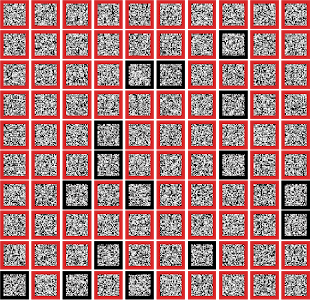
\includegraphics[width=0.9\textwidth]{images/Motivation/pred_noise.png}
    \caption{A model trained to recognize MNIST digits often makes strong predictions over random noise. For each red square, this typical models softmax output gives over $0.5$ confidence in one of the ten digits, i.e. a majority of the confidence.}
    \label{fig:mot-pred-noise}
\end{figure}\\
The curse of dimensionality refers to many unintuitive phenomena that arise when analyzing data in high-dimensional spaces. Notably, distances become hard for humans to visualize. \ref{fig:mot-dist} shows a simplistic example. Other commonly referenced unintuitive phenomena are that high-dimensional spheres have most of their volume concentrated near their surface, and that high-dimensional data sets become easier to linearly separate.
\begin{figure}[!htbp]
    \centering
    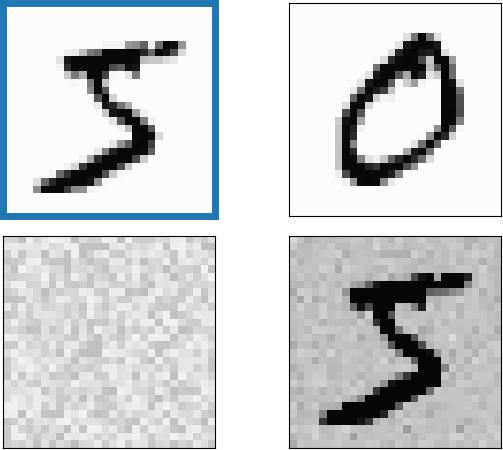
\includegraphics[width=0.9\textwidth]{images/Motivation/motivation-distances.png}
    \caption{Three distinct images that all have the same Euclidean distance from the image in the blue box. Human perception doesn't always align with mathematical definitions.}
    \label{fig:mot-dist}
\end{figure}\\
The combination of the piece-wise linearity of neural networks with the various unintuitive curse of dimensionality phenomena lead to various unexpected behaviors of the networks. For example Szegedy et.al.\cite{szegedy2013intriguing} showed that the boundaries between the various classes in the hyper-space (as predicted by a neural network) are often linear and close distance-wise. \ref{fig:mot-bounds} shows an example of this behavior.
\begin{figure}[!htbp]
    \centering
    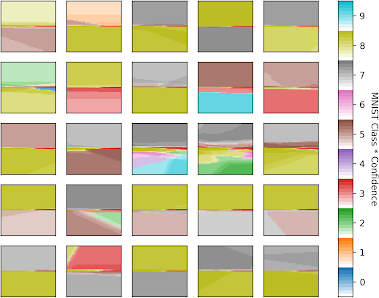
\includegraphics[width=0.9\textwidth]{images/Motivation/boundaries.png}
    \caption{What this simple MNIST model predicts when moving along an image-to-image vector. Each pixel represents point in the MNIST image 748 dimensional space, with centre-leftmost pixels and centre-rightmost pixels being two images pulled from the data. Left-right movement along the center corresponds to linear compositions of the two images. Each vertical axis corresponds to movement along a different random vector orthogonal to the left-right image-to-image vector. Each color corresponds to an MNIST class prediction. Surprisingly, while the two images are correctly classified as 8 and 3 respectively, orthogonal movement almost always ends leads to a different class. An analogy would be: walking in a straight line from Paris to Berlin predictably takes you from France to Germany, and might cross any number of other countries, but any step left or right of that straight line always lands outside of France or Germany. }
    \label{fig:mot-bounds}
\end{figure}\\
These intuitions motivate the definition of the Finite Gaussian Neuron (in \ref{Definition of the Finite Gaussian Neuron}), as a combination of a classical neuron with a Gaussian of finite range. 


\section{Related Work}
% \subsection{Fast Gradient Sign Method}
% \subsection{Adversarial Training}
In the paper by Goodfellow et al.\cite{goodfellow2015explaining} introducing adversarial attacks, it is shown that continuous retraining of the model using adversarial examples protects the model from attacks. This adversarial training method however is computationally expensive as it requires both creating new adversarial examples after each training epoch and continuously retraining the model with a potentially growing dataset. It is also shown that adversarial training based on the Fast Gradient Sign Method (FGSM) of the paper does not necessarily protect against other adversarial attacks.\\
Pushing adversarial training further, Madry et al.\cite{madry2019deep} show that the Project Gradient Descent (PGD) attack provides adversarial examples that may well generalize to other gradient based attacks. However this potential universal robustness again first-order attacks requires larger networks. In addition PGD, as an iterated FGSM attack, is especially computationally expensive.\\
%\subsection{Distillation}
Another proposed defense against adversarial attacks is Distillation, proposed by Papernot et al. \cite{Papernot2016DistillationAA}. Originally designed as a method to reduce the size of DNNs by transferring knowledge from larger to smaller networks. Distillation works by training a large network, then using the output prediction vectors as soft-labels to train a smaller network, encoding class similarities in the soft-labels. Instead of aiming to reduce model size, the authors show that retraining the same model on the soft-labels provides defense against adversarial attacks by making the network less sensitive to small changes over the input, and requiring a higher average minimum
number of features to be modified in order to create adversarial examples. Similarly to adversarial retraining, distillation requires additional computation to generate the soft-labels and retrain the model.\\
% \subsection{Radial Basis Function Networks}
Radial Basis Function (RBF) networks have also been explored as a more intrinsic defense against rubbish data and adversarial attacks\cite{chenou2019radial,zadeh2018deeprbf} and in fact are similar in many ways to the Finite Gaussian Neuron networks. However they have not become as popular as other deep neural networks techniques, perhaps due to their complexity. The RBF architecture doesn't easily generalize to multiple layers, and requires pre-processing work to properly place the prototypes.


\chapter{The Finite Gaussian Neuron}
A classical artificial neuron's activity $y_c$ is defined by: 
\[ y_{c} = \varphi(\ell) \]
\[ \ell = \sum_{i}w_i x_i\]
with $\ell$ being the linear component defined by linear combination of the inputs $x_i$ and associated weights $w_i$, and with $\varphi$ being the non-linear activation function required by the universal approximator theorem \cite{cybenko1989approximation, hornik1989multilayer}. The bias term can be added explicitly or implicitly included as an extra input with value 1. \ref{fig:classic-neuron} gives a visualization of this classical neuron. 
\begin{figure}[!htbp]
    \centering
    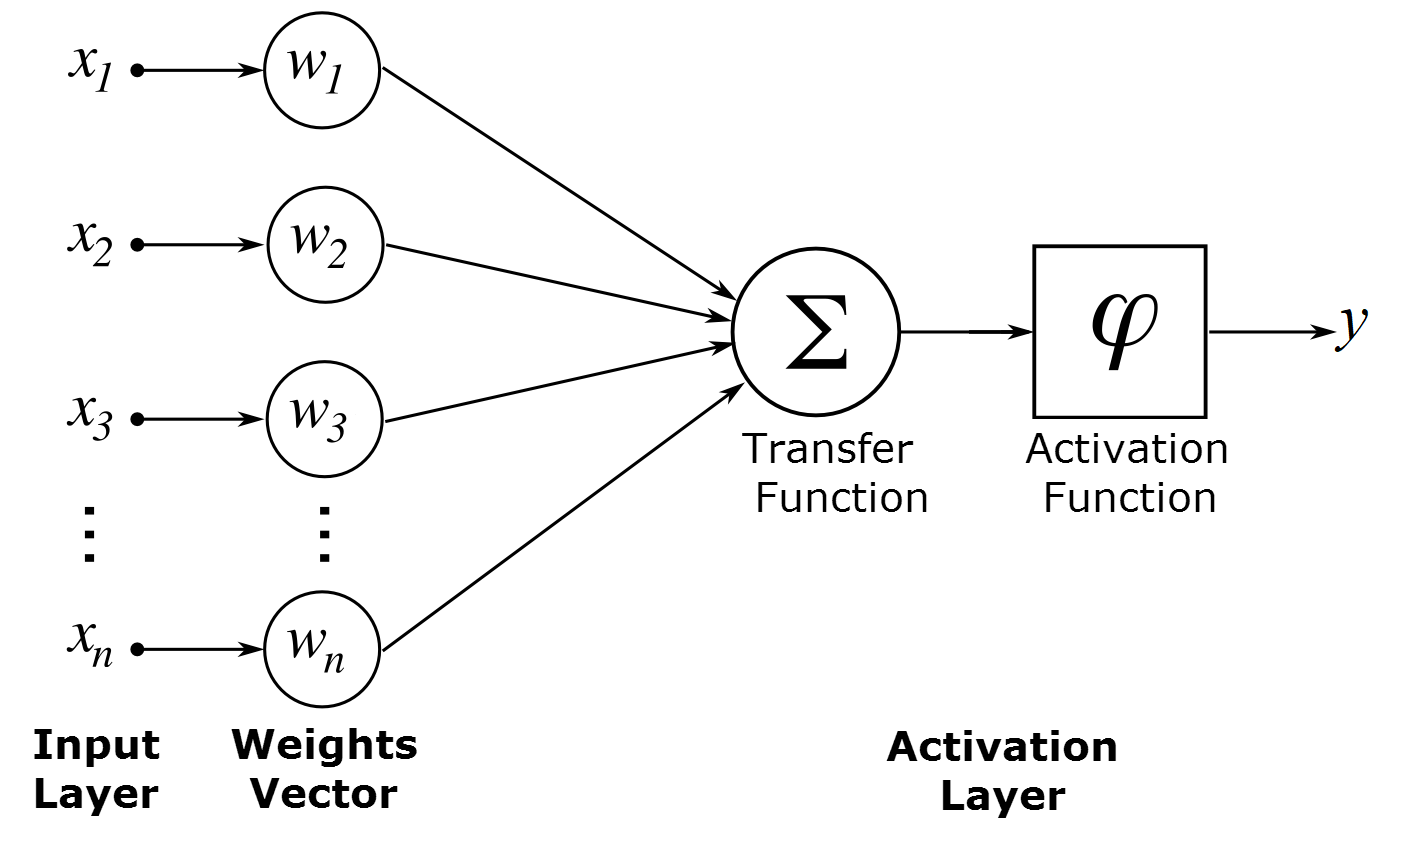
\includegraphics[width=0.9\textwidth]{images/artificial_neuron_model.png}
    \caption{A classical representation of the artificial neuron.}
    \label{fig:classic-neuron}
\end{figure}\\

\section{Definition of the FGN} \label{Definition of the Finite Gaussian Neuron}
I introduce the Finite Gaussian Neuron (FGN) as a combination of the classical neuron's activity with a Gaussian activity that limits the range of the neuron. Explicitly, the FGNs output $y_f$ is given by:
\[y_{f} = \varphi(\ell) * g\]
\[g = e^{\frac{-1}{\sigma^2}\sum_{i}(x_i-c_i)^2}\]
with $\ell$ and $\varphi$ the same as the classical neuron i.e. the linear component and non-linear activation function respectively; and with $g$ the new Gaussian component, defined by centers $c_i$ that position the neuron in the input hyperspace, and range $\sigma$ that gives the neuron a limited range. If inputs are far away from the center, relative to the range $\sigma$, then the Gaussian component $g$ will have value zero and the FGN's output activity will be zero as well, thus limiting the range of neurons to a finite zone of the input hyperspace. \ref{fig:gaussian-comp} shows a visualization of the new Gaussian component G.
\begin{figure}[!htbp]
    \centering
    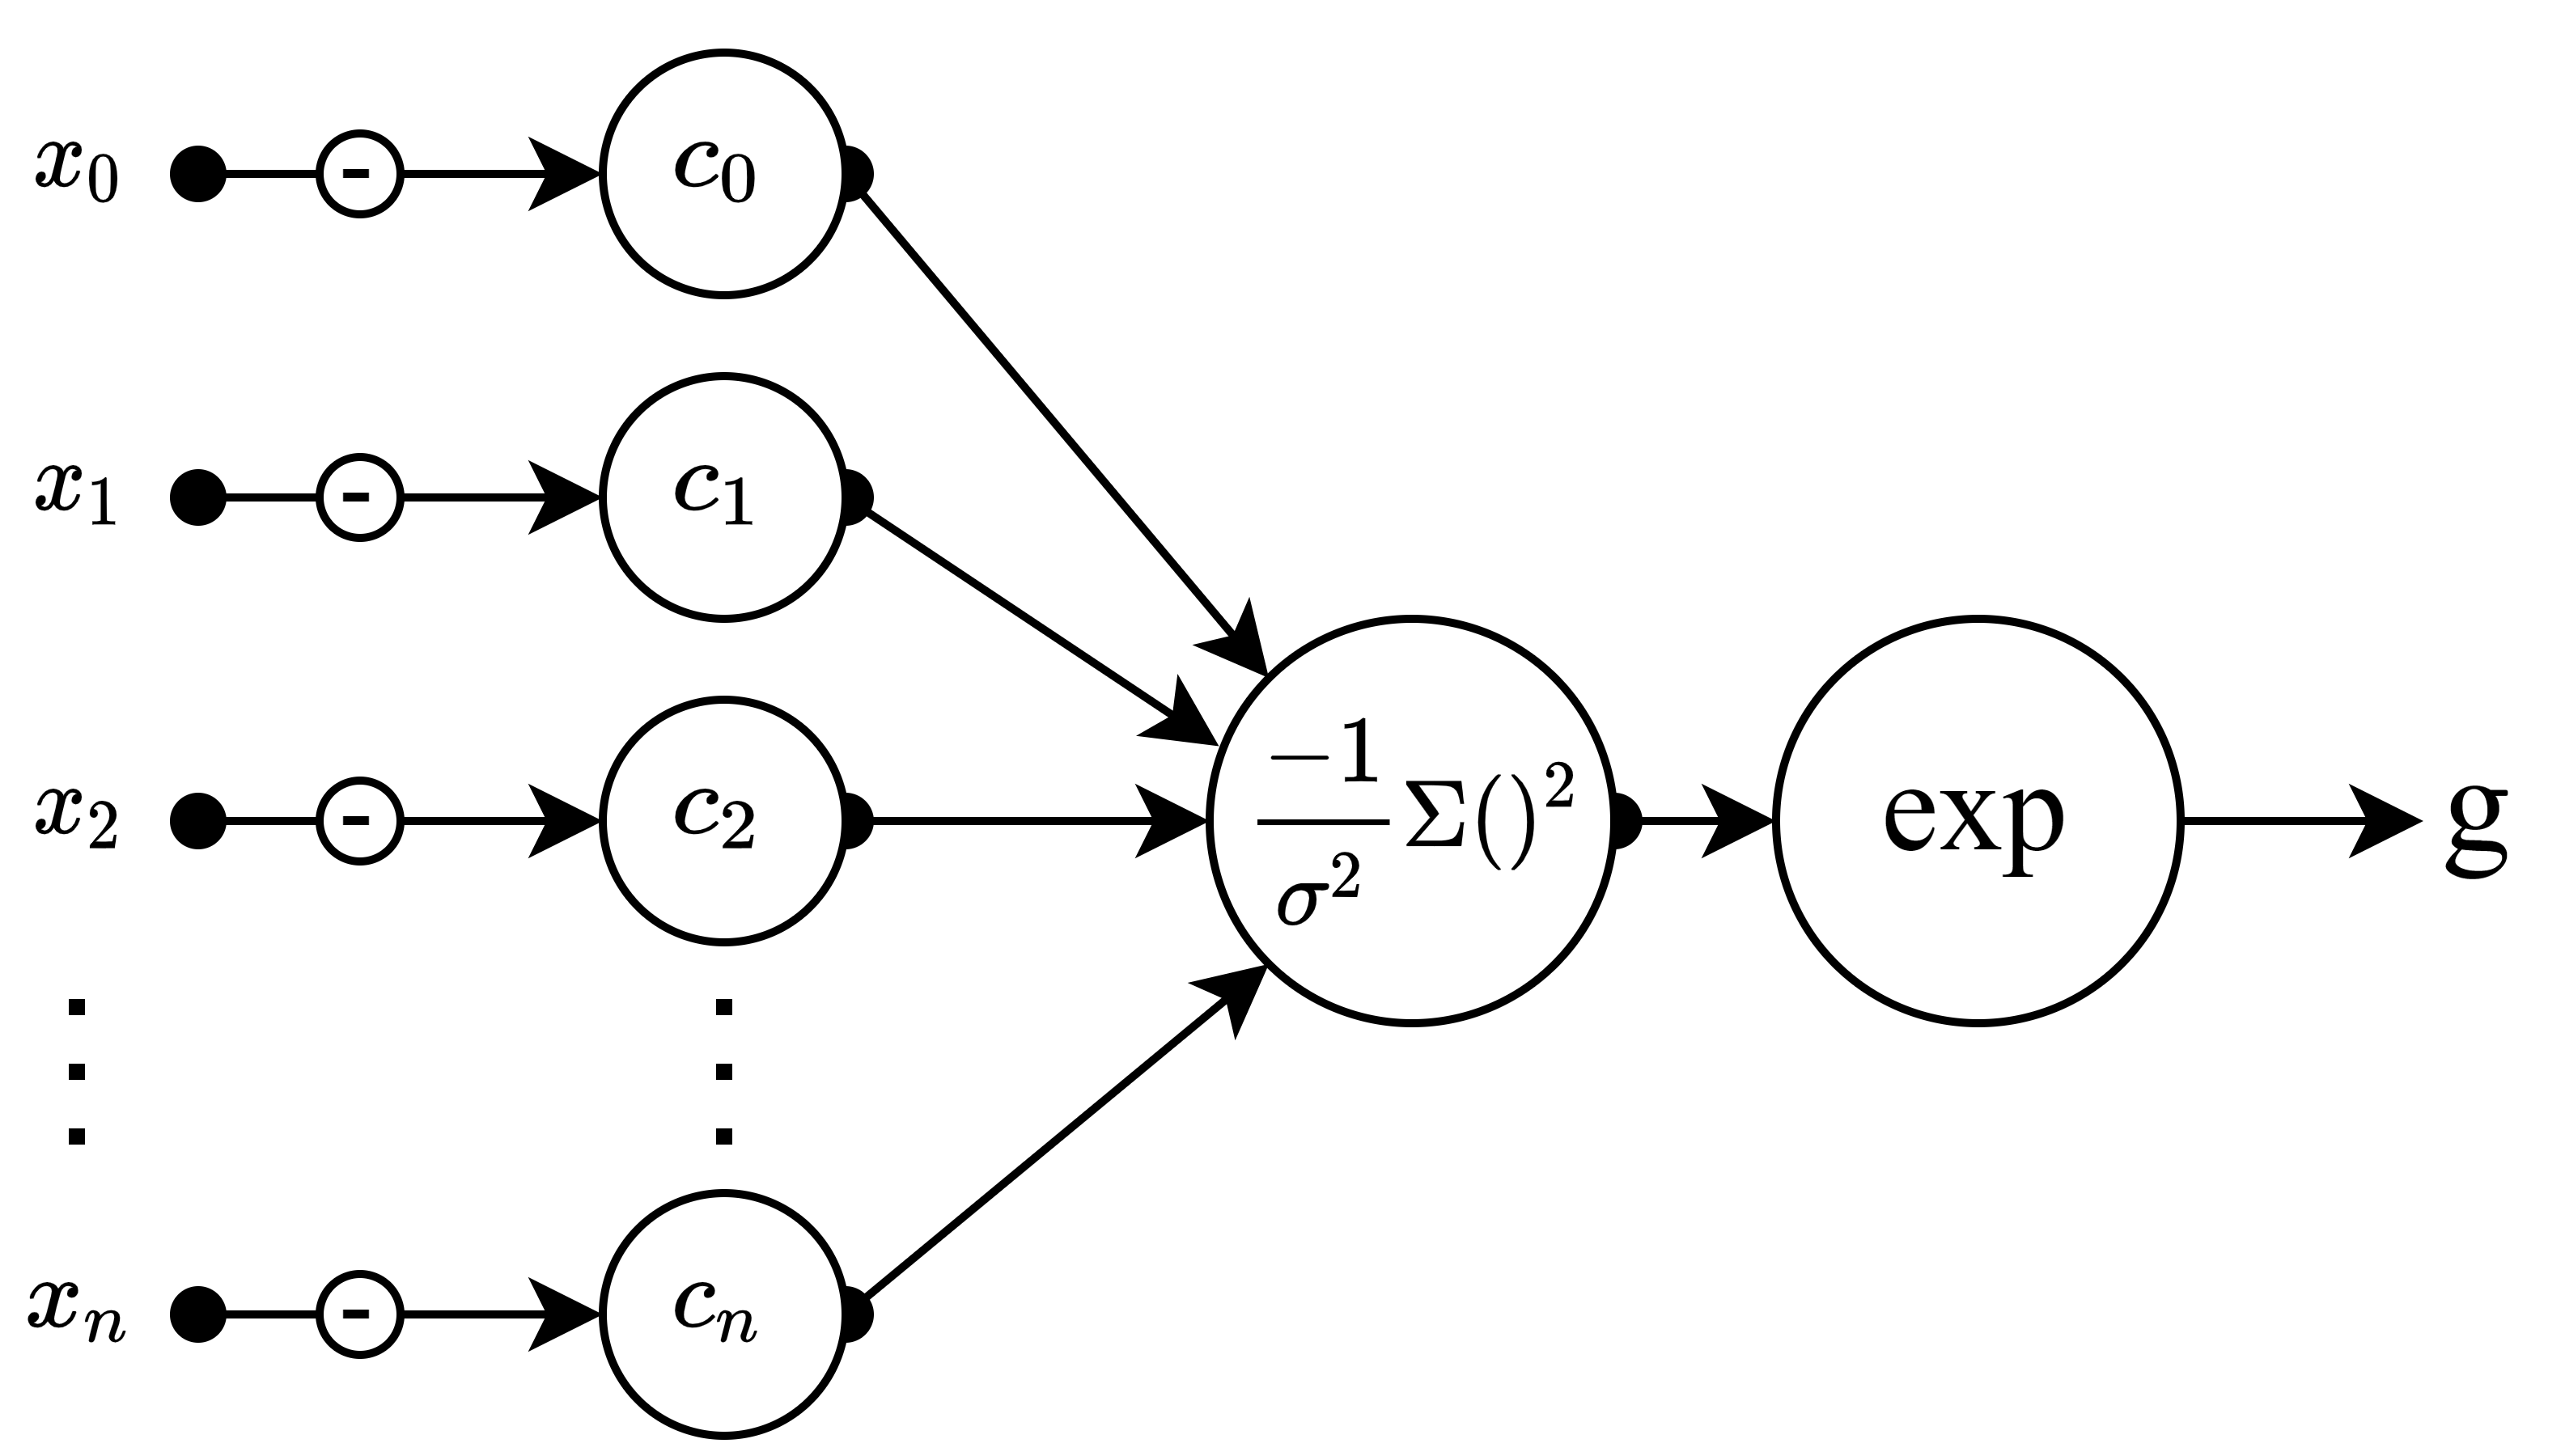
\includegraphics[width=0.9\textwidth]{images/fgn-gaussian-component.png}
    \caption{The Gaussian component of an FGN.}
    \label{fig:gaussian-comp}
\end{figure}\\
% visuals
The following figures (\ref{fig:classic-heatmap}, \ref{fig:fgn-heatmap}) show the difference in behavior between the classic neuron architecture and the FGN architecture, for an arbitrary neuron, over a two dimensional input space.
\begin{figure}[!htbp]
    \centering
    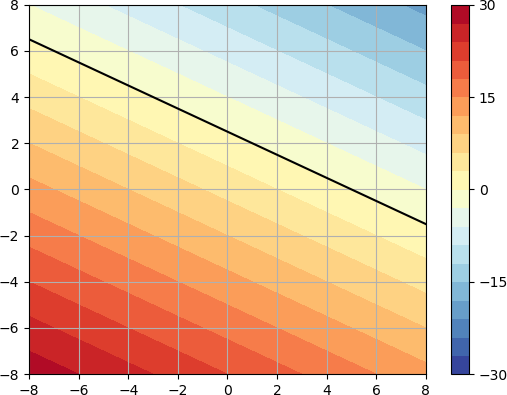
\includegraphics[width=0.49\textwidth]{images/2D Activity/2d-linear-activity-cropped.png}
    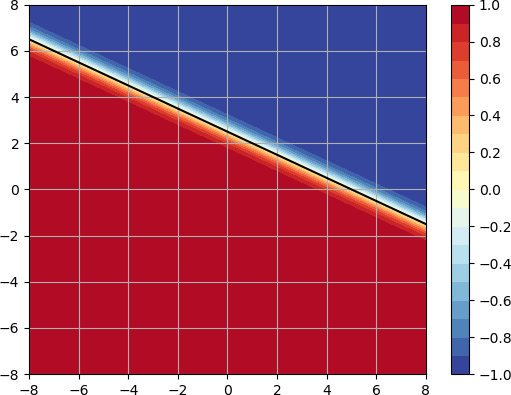
\includegraphics[width=0.49\textwidth]{images/2D Activity/2d-classic-activity-cropped.png}
    \caption{On the left, the $\ell = \sum_{i}w_i x_i$ linear component of the classical neuron architecture with arbitrary weights, shown as an activity heatmap over a 2-d input space. On the right the same neuron's output $y_c = \tanh(\ell)$  after the linear component is passed through the typical $tanh$ non-linear activation function. The black line shows where the heatmap value is zero.} 
    \label{fig:classic-heatmap}
\end{figure}\\
\begin{figure}[!htbp]
    \centering
    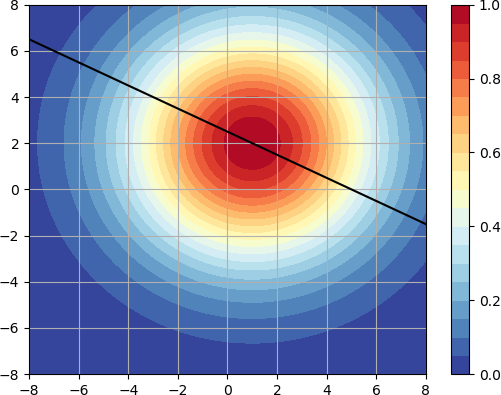
\includegraphics[width=0.49\textwidth]{images/2D Activity/2d-gaussian-activity-cropped.png}
    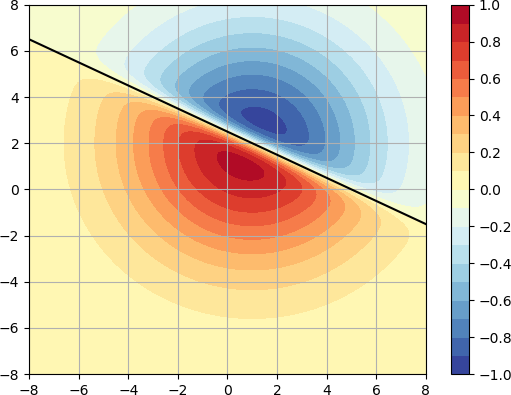
\includegraphics[width=0.49\textwidth]{images/2D Activity/2d-fgn-activity-cropped.png}
    \caption{On the left, the $g = e^{\frac{-1}{\sigma^2}\sum_{i}(x_i-c_i)^2}$ Gaussian component of the FGN architecture with arbitrary centers and range, shown as an activity heatmap over a 2-d input space. The zero line is only for comparison with the in \ref{fig:classic-heatmap} linear component above. On the right, the FGN's output $y_f = \tanh(\ell) * g$ combining the output of the classical neuron with the Gaussian component. Note the finite range of the FGN's activity.}
    \label{fig:fgn-heatmap}
\end{figure}\\
% desired behavior
The desired outcome of defining the FGN in this way is to restrict the activity of the neural network to  regions of the input hyperspace where data has been observed during training, while making no guess over regions never observed. And, if this works as intended, adversarial examples will be harder to find.\\

\section{Classic Neuron Conversion to FGN}
One important property of the FGN is that existing networks using the classical neuron architecture can be converted to the FGN architecture without changing the network's behavior over given data. This is done by converting each classical neuron in the original network to an FGN with identical weight vector $W$ and large range $\sigma$. Figure \ref{fig:matching} illustrates this property.
\begin{figure}[!htbp]
    \centering
    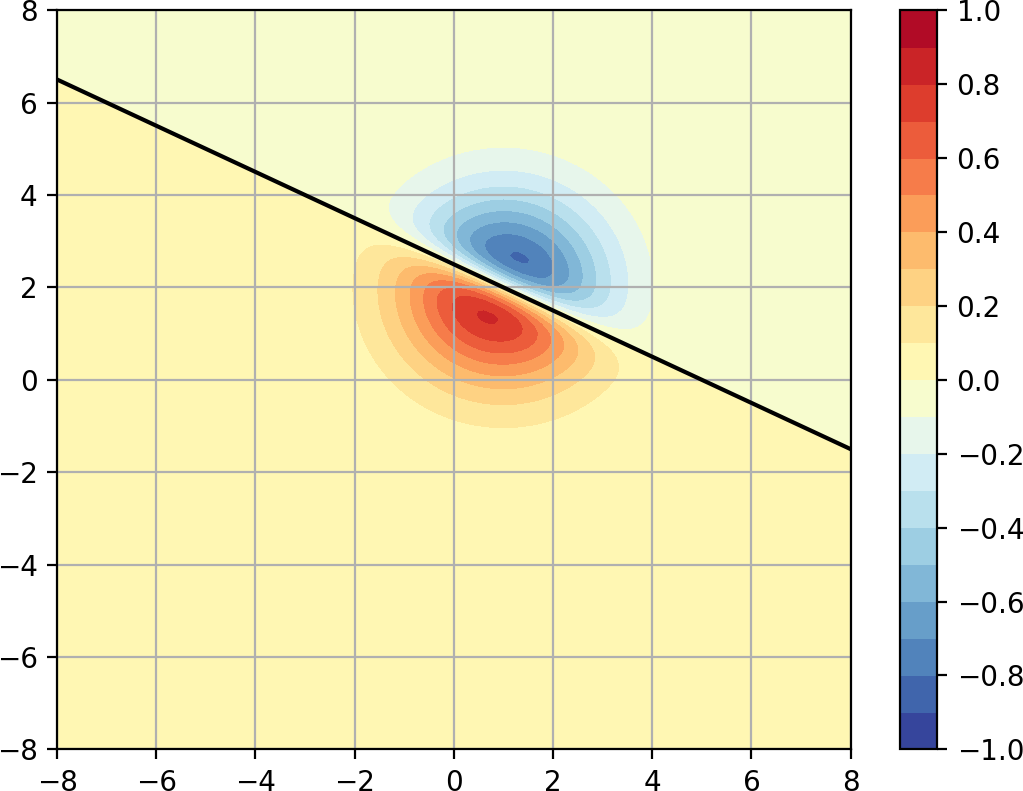
\includegraphics[width=0.32\textwidth]{images/Matching-behavior/sigma-2-cropped.png}
    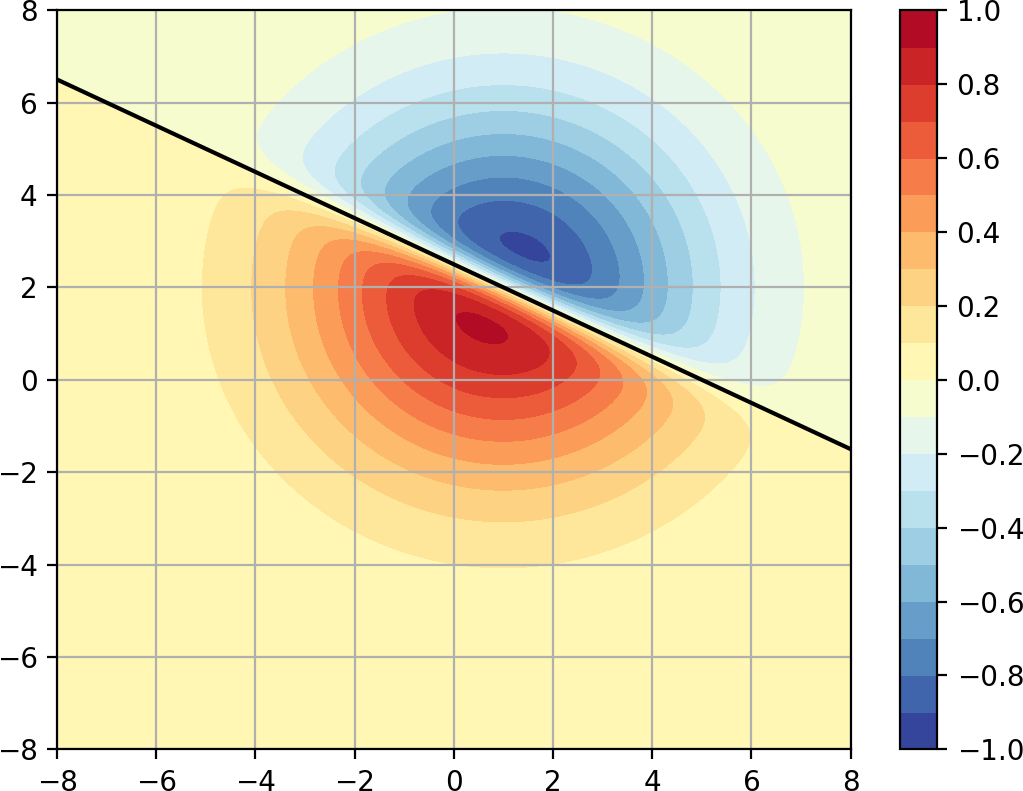
\includegraphics[width=0.32\textwidth]{images/Matching-behavior/sigma-3-cropped.png}
    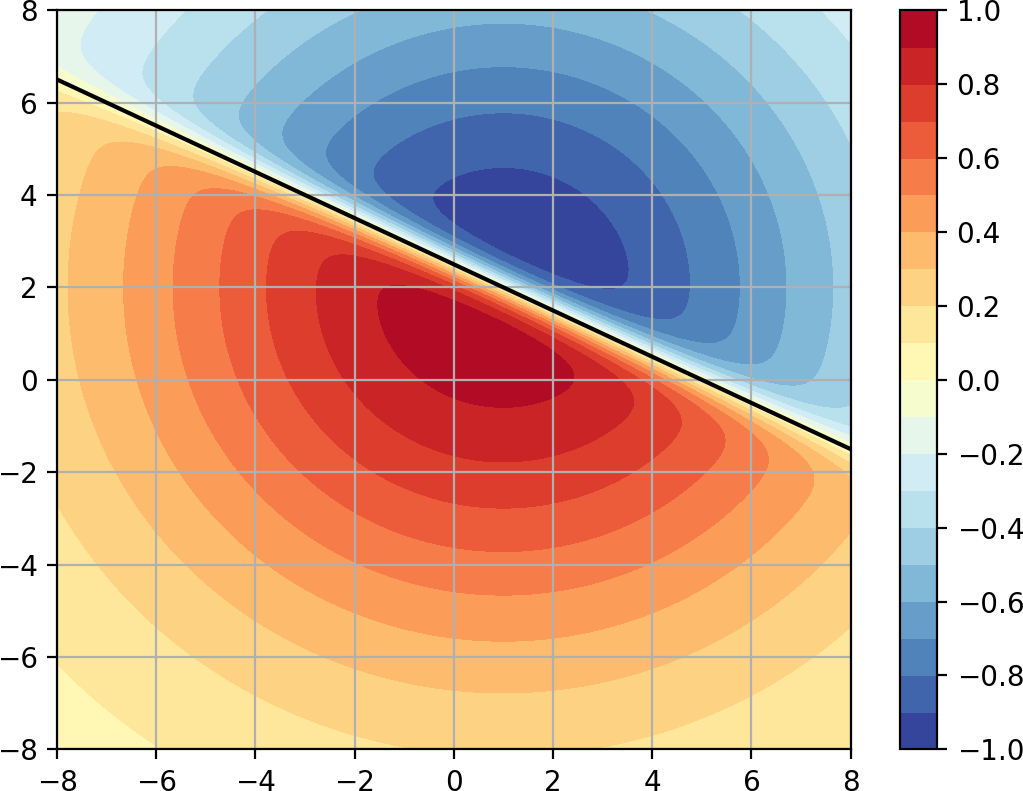
\includegraphics[width=0.32\textwidth]{images/Matching-behavior/sigma-4-cropped.png}
    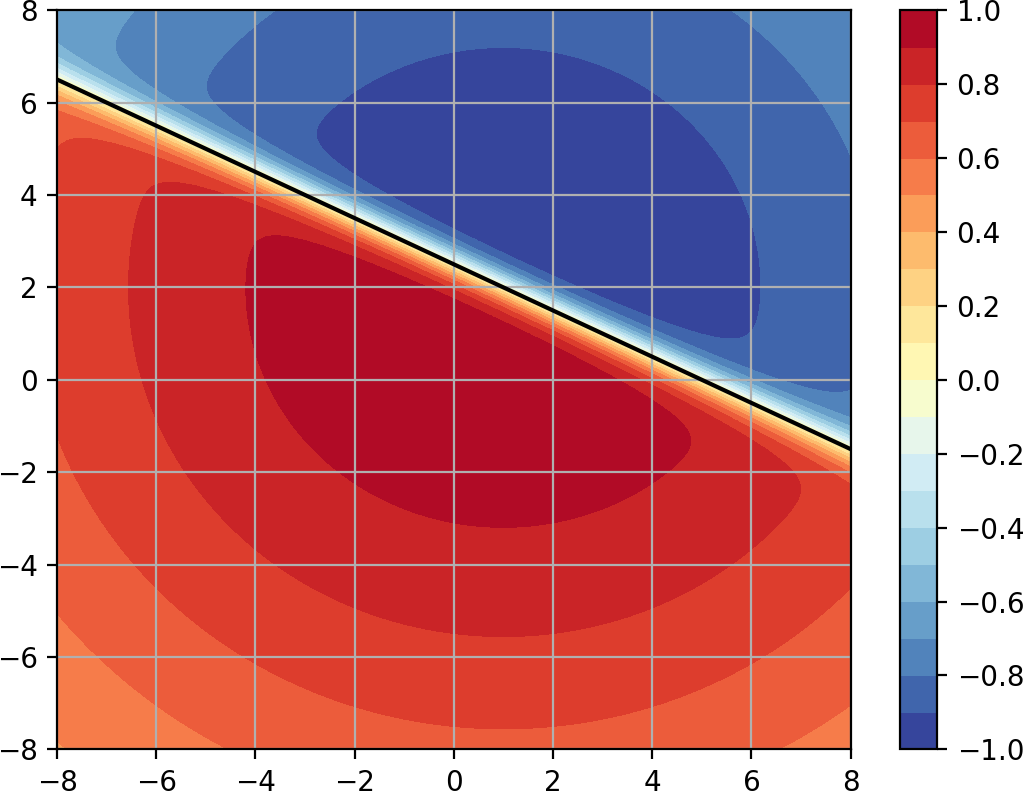
\includegraphics[width=0.32\textwidth]{images/Matching-behavior/sigma-5-cropped.png}
    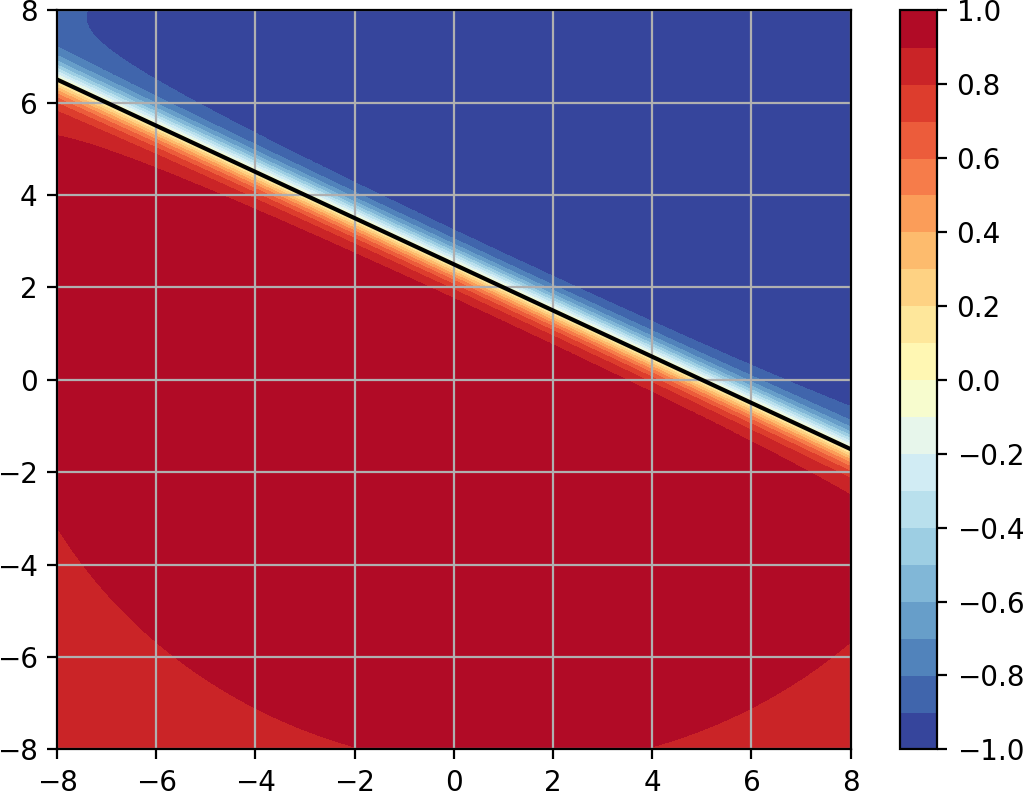
\includegraphics[width=0.32\textwidth]{images/Matching-behavior/sigma-6-cropped.png}
    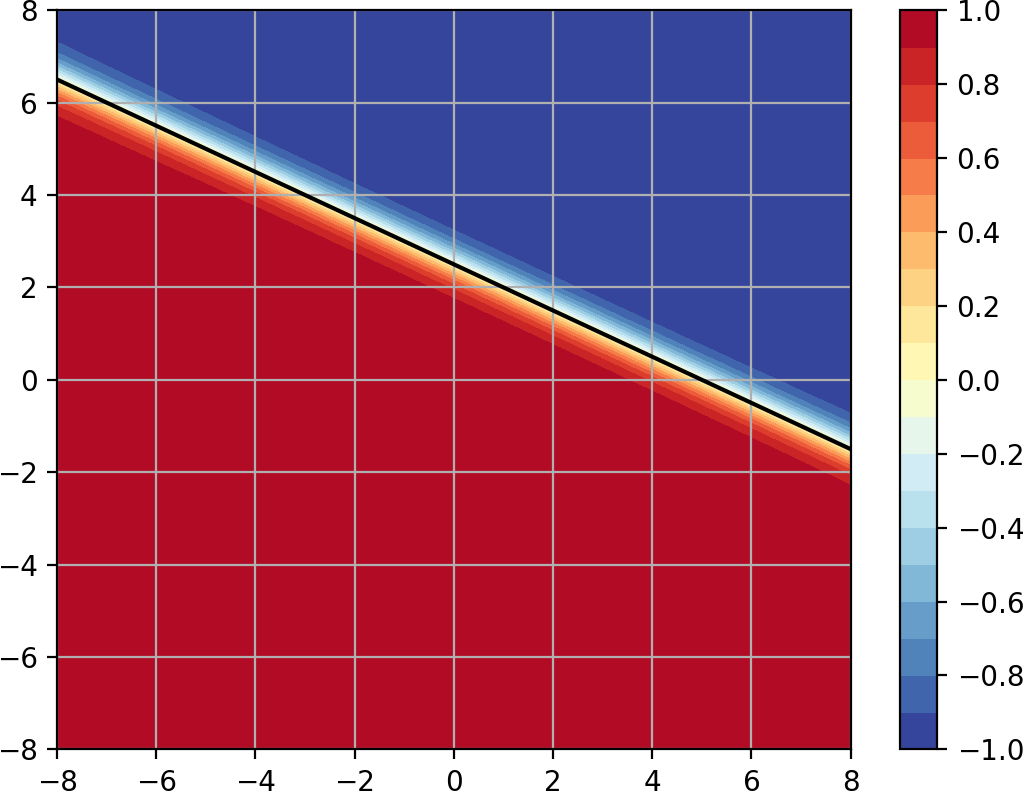
\includegraphics[width=0.32\textwidth]{images/Matching-behavior/sigma-7-cropped.png}
    \caption{Illustration showing that increasing an FGN's range $\sigma$ (smallest top-left, largest bottom-right) leads to behavior identical to that of classical neuron with the same weights $W$. Note how the final picture is indistinguishable that shown in figure \ref{fig:classic-heatmap}. }
    \label{fig:matching}
\end{figure}\\
Converting a classical neuron to an FGN involves defining two new parameters, the range $\sigma$ and the centers $c_i$. For any given dataset, there will be a unique $C=c_i$ that allows for minimum valued range while not changing the behavior over this dataset, but finding this center is not trivial, and the topic of future research. Currently, conversion is done by setting the center $C$ to be the point on zero line (defined by the neuron weights $W$) closest to the origin, and empirically searching for a range $\sigma$ large enough.

\section{Training the FGN}
Training the FGN is done much the same way as the classical neuron: we find parameters of the FGN that locally minimize a cost function using using the back-propagation algorithm. So far, experiments have not shown any specific loss function (Mean-Squared Error, Cross-Entropy, etc...) or gradient descent optimizer algorithm (Adam, RMSprop, etc...) to perform any differently on FGNs versus classical neurons. \\
Since one of the goals of the FGN is to limit the activity far from the data, we add a regularization term $\lambda$ to the loss function $\tilde{C}$ to add pressure to minimize the range $\sigma$ during training. $\lambda$ becomes a hyper-parameter of the neuron to tune to the task like any other hyper-parameter.\\
\[C = \tilde{C} + \lambda\sigma^2\]
The precise gradients depend on the cost $C$ and non-linear activation $\Phi$ functions chosen, but the partial derivatives of the FGN output $y$ for an input $x_i$  are:
\begin{align*}
    \text{Weights:\quad} \frac{\partial y}{\partial w_i} &=  x_i \varphi'(\ell) * g  \\[1em]
    \text{Centers:\quad} \frac{\partial y}{\partial c_i} &= \varphi(\ell) * \frac{2(x_i-c_i)}{\sigma^2} * g \\[1em]
    \text{Sigmas:\quad} \frac{\partial y}{\partial \sigma} &= \varphi(\ell) * \frac{2\sum_{i}(x_i-c_i)^2}{\sigma^3}* g
    % \text{(Reminder:\quad} y &=  \varphi(\ell)*g = \tanh(\sum_i x_i w_i) * e^{\frac{-1}{\sigma^2}\sum_{i}(x_i-c_i)^2} )
\end{align*}
The changes to each of the parameters all depend in part on the Gaussian component $g$. In particular they all need it to be non-zero or they will not change. This shows that the FGN can only learn when the input is close to the neuron centers $c_i$ relative to the range $\sigma$. Proper initialization is thus important, to ensure that the FGN range and centers cover the data, else the gradients will be non-existent. \\
\indent As a sanity check, I verified that a single FGN is able to be trained to properly classify a two dimensional linearly separable toy dataset, show in figure \ref{fig:single-fgn-1}. The following figures \ref{fig:single-fgn-2}, \ref{fig:single-fgn-3} show the FGN's weights $W$, centers $c_i$ and range $\sigma$ adapting to fit the data.
\begin{figure}[!htbp]
    \centering
    \hspace{0.0\textwidth}
    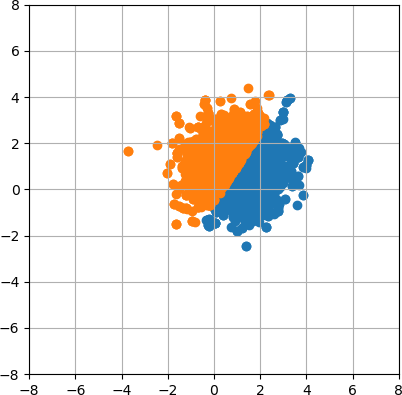
\includegraphics[width=0.405\textwidth]{images/2D-single-neuron/2d-easy-data-cropped.png}
    \hspace{0.04\textwidth}
    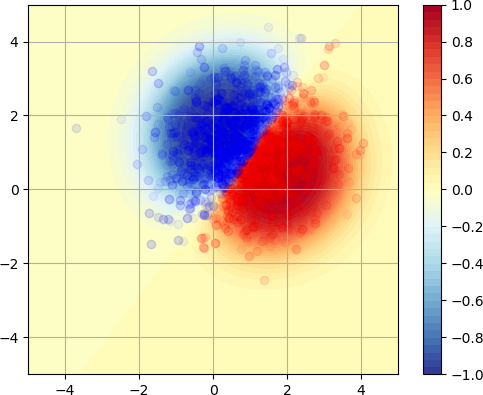
\includegraphics[width=0.49\textwidth]{images/2D-single-neuron/2d-easy-trained-activity-cropped.png}
    \caption{The 2D linearly separable toy data centered on $(1,1)$, and the activity of the FGN over the space after training with MSE cost function, $\lambda=0.01$ range $\sigma$ regularization term, Adam optimizer with $lr=0.05$.}
    \label{fig:single-fgn-1}
\end{figure}
\begin{figure}[!htbp]
    \centering
    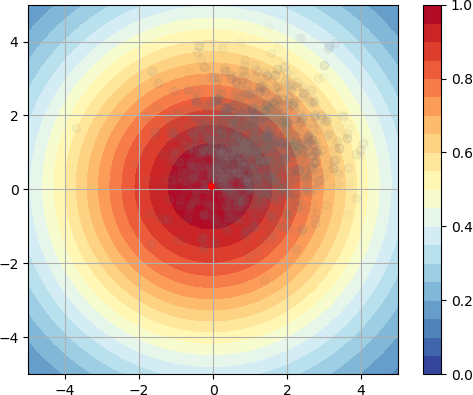
\includegraphics[width=0.49\textwidth ]{images/2D-single-neuron/2d-easy-initialg-cropped.png}
    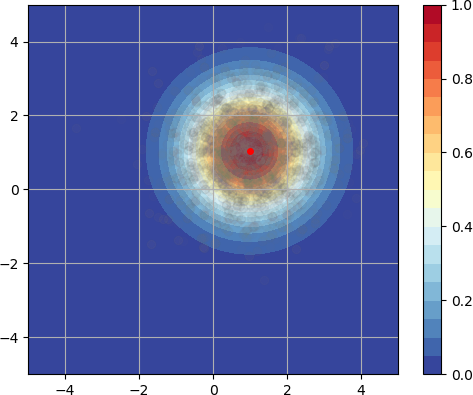
\includegraphics[width=0.49\textwidth]{images/2D-single-neuron/2d-easy-trainedg-cropped.png}
    \caption{The FGN's Gaussian component $g$ activity over the 2D space pre and post training. Initially centered on the origin $(0,0)$ with range $\sigma=5$, after training the Gaussian component is centered on the data and the range has shrunk such that space far from the data has $g=0$ activity.}
    \label{fig:single-fgn-2}
\end{figure}\\
\begin{figure}[!htbp]
    \centering
    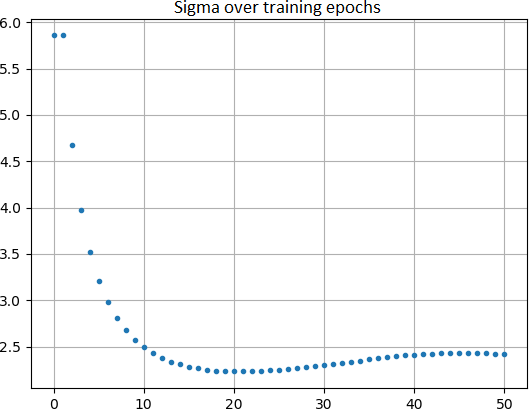
\includegraphics[width=0.49\textwidth,height=6.35cm]{images/2D-single-neuron/2d-easy-sigma-training-cropped.png}
    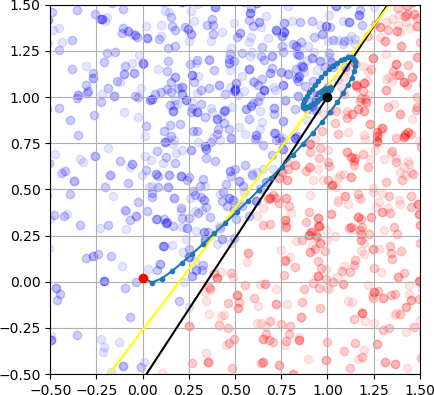
\includegraphics[width=0.49\textwidth]{images/2D-single-neuron/2d-easy-center-path-cropped.png}
    \caption{Evolution of the FGN's range $\sigma$ and center position during training. On the left, pressured by the cost function's regularizer term, $\sigma$ shrink as much as possible while still fitting the data.  On the right, the dotted blue line shows the FGN center's path during training, starting from the red dot in $(0,0)$ and moving towards the theoretically optimal center $(1,1)$ (black dot). The black line is the class border and the yellow line is the FGN's predicted border, given by the weights $W$.}
    \label{fig:single-fgn-3}
\end{figure}

\section{Alternative Implementations}
There are several implementation alternatives that may improve the FGN's performance on specific tasks. 
\indent An FGN built to match the behavior of a classical neuron will define the bias term of the linear component $\ell$ by the centers of the FGN, so that the line of zero activity for the linear component passes through the center. This isn't strictly needed when retraining the FGN or when training from scratch. Figure \ref{fig:decoupled} is an example of an FGN with decoupled bias and centers in two dimensional input space. All the experiments performed in later sections were done with decoupled bias and centers.
\begin{figure}[!htbp]
    \centering
    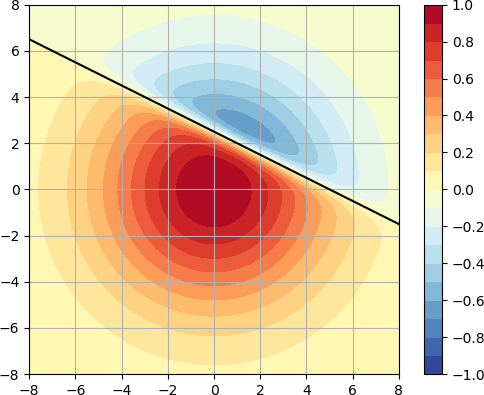
\includegraphics[width=0.66\textwidth]{images/2D-Decoupled/var-decoupled-center-activity-cropped.png}
    \caption{Activity of an FGN with a decoupled bias and centers.}
    \label{fig:decoupled}
\end{figure}\\
\indent Since distances in higher dimensions are harder to grasp, various norms for the Gaussian component $g$ were considered over the Euclidean norm.
\[g = e^{\frac{-1}{\sigma^2}\lVert x_i-c_i \lVert_p }\]
Figure \ref{fig:norms} shows how changing the ordinal $p$ of the norm affects the FGN's output, visualized over a two dimensional input space. Cursory experiments have not shown any differences in FGN performance between the various $p$-norms, and the Euclidean norm was used.
\begin{figure}[!htbp]
    \centering
    \begin{subfigure}[t]{0.32\textwidth}
        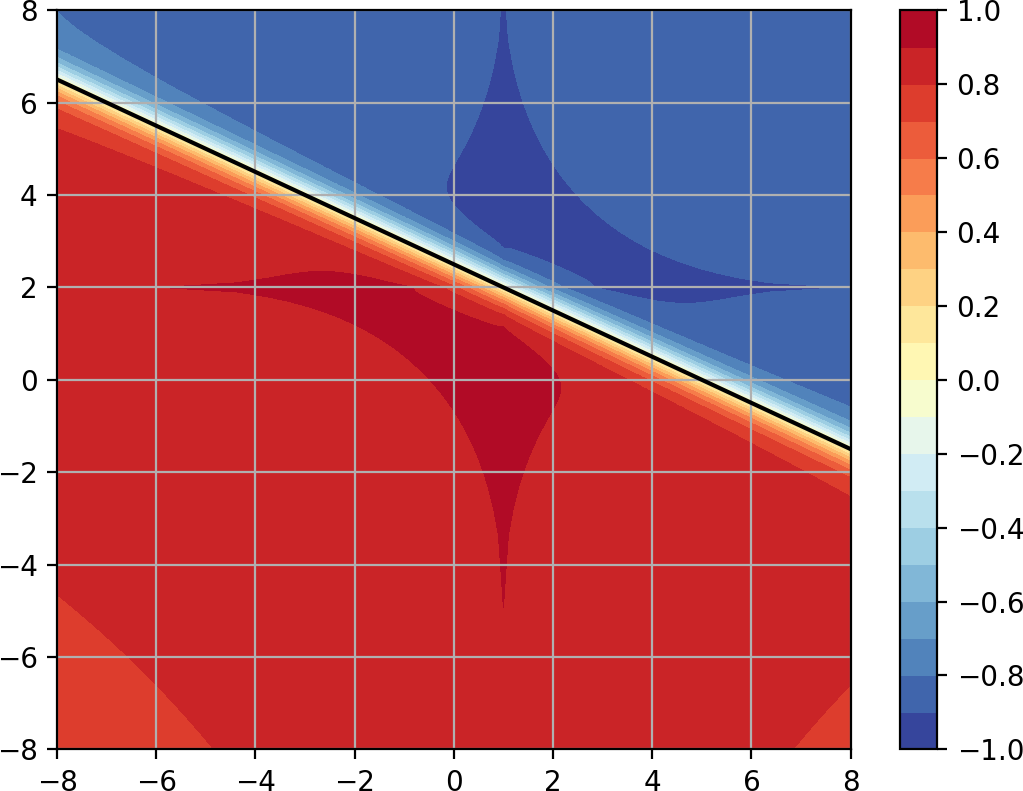
\includegraphics[width=\textwidth]{images/Variants-Norms/ord0.5-cropped.png}
        \caption*{$p=0.5$}
    \end{subfigure}
    \begin{subfigure}[t]{0.32\textwidth}
        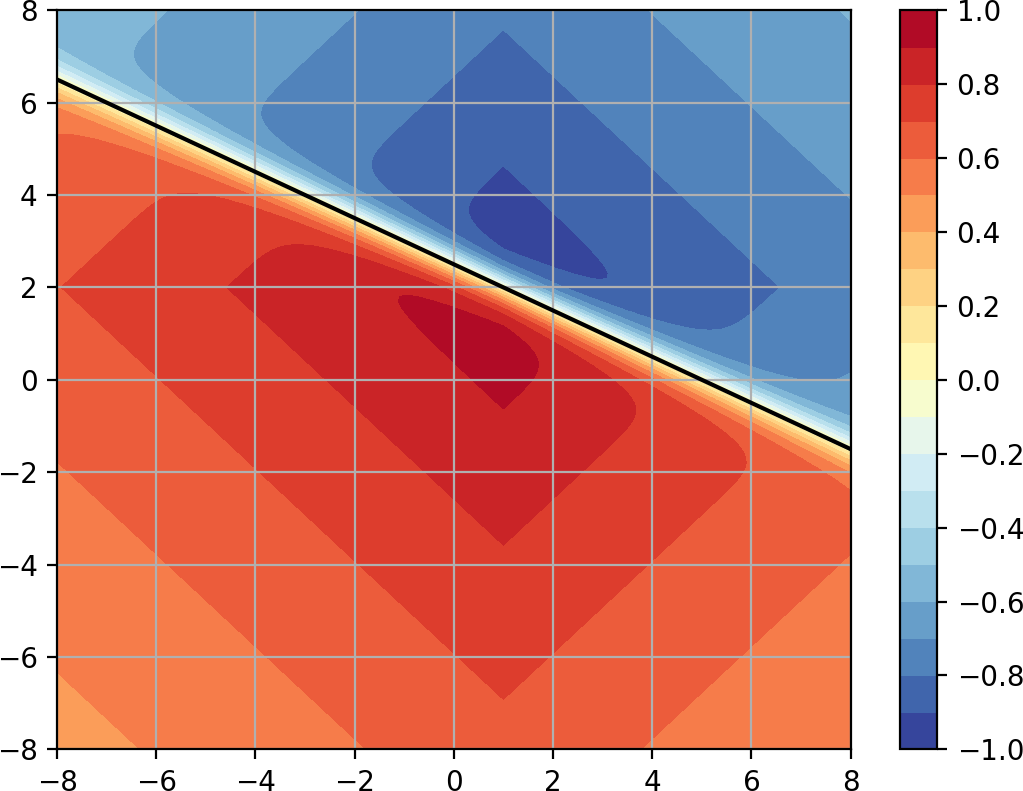
\includegraphics[width=\textwidth]{images/Variants-Norms/ord1-cropped.png}
        \caption*{$p=1.0$}
    \end{subfigure}
    \begin{subfigure}[t]{0.32\textwidth}
        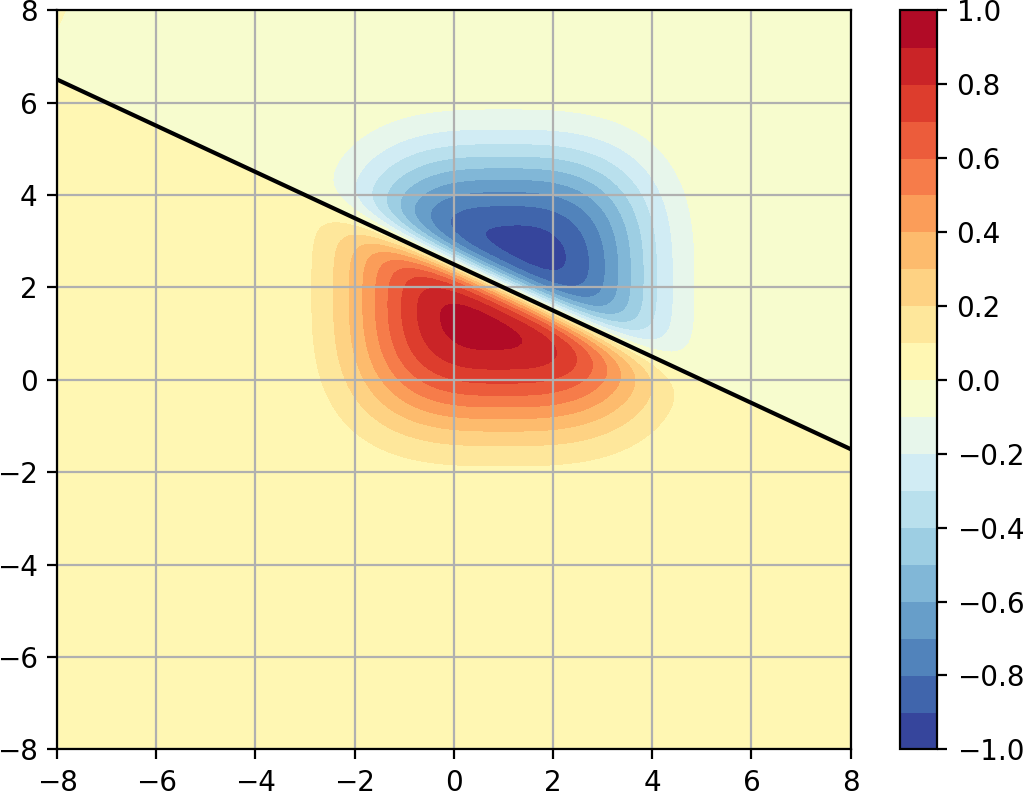
\includegraphics[width=\textwidth]{images/Variants-Norms/ord3-cropped.png}
        \caption*{$p=3.0$}
    \end{subfigure}
    \caption{Examples of how the $p$-norm of the FGN's Gaussian component affects activity.}
    \label{fig:norms}
\end{figure}\\
\indent The range term $\sigma$, which defines how large or small the (hyper-)sphere of activity is for the Gaussian component $g$, can be modified into a matrix $\Sigma$ to stretch and/or rotate the sphere into an ellipse, which gives the FGN a different range along each of its inputs.\\
The Gaussian component $g$ then becomes
\[g = e^{-(X-C)^T * \Sigma^{-1} * (X-C)}\]
with $X=[x_i]$ the inputs vector, $C=[c_i]$ the centers vector and $\Sigma$ the range covariance matrix (semi-definite positive). Figure \ref{fig:covars} gives examples of such $\Sigma$ matrices. Note that a full $\Sigma$ matrix has $N^2=$ elements, with $N$ being the number of inputs to the FGN, making the computation of $g$ intractable for any larger problem. A diagonal $\Sigma$ matrix is feasible.
\begin{figure}[!htbp]
    \centering
    \begin{subfigure}[t]{0.49\textwidth}
        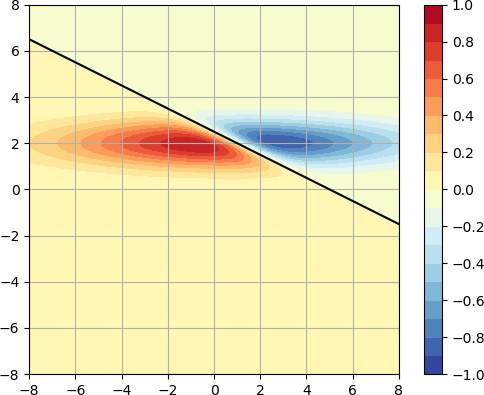
\includegraphics[width=\textwidth]{images/Variants-Diag-Full-Cov/diag_full_activity_cropped.png}
        \caption*{Diagonal $\Sigma$}
    \end{subfigure}
    \begin{subfigure}[t]{0.49\textwidth}
        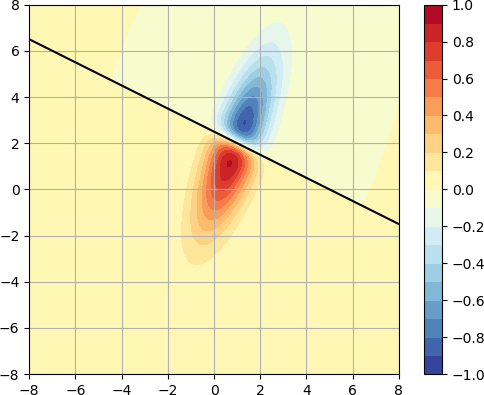
\includegraphics[width=\textwidth]{images/Variants-Diag-Full-Cov/full_full_activity_cropped.png}
        \caption*{Full $\Sigma$}
    \end{subfigure}
    \caption{Examples of how using a range $\Sigma$ matrix allows the FGN to consider changes along one input dimension to be important than another.}
    \label{fig:covars}
\end{figure}

\section{Multi-Layer FGN Networks}
Extending the FGN architecture to neural networks is straightforward save for one detail: the Gaussian component $g$ needs to consider the Gaussian components of the previous layer to be able to propagate out-of-range activities. Without this Gaussian gate, activity far from the data defaults to an arbitrary value, not necessarily to zero as desired. A layer $j$ FGN's output $y$ is given by
\[y =  \varphi(\ell)*g = \varphi(\sum_i x_{i} w_{i}) * g\]
\[g = \max(G_{j-1}) * e^{\frac{-1}{\sigma^2}\sum_{i}(x_i-c_i)^2}\]
With $x_{i}$ and $G_{j-1}$ the previous layer outputs and Gaussian components. For the initial layer, $\max(G_{j-1})$ should be set to $1$. Figure \ref{fig:fgn-layer} illustrates this process.
\begin{figure}[!htbp]
    \centering
        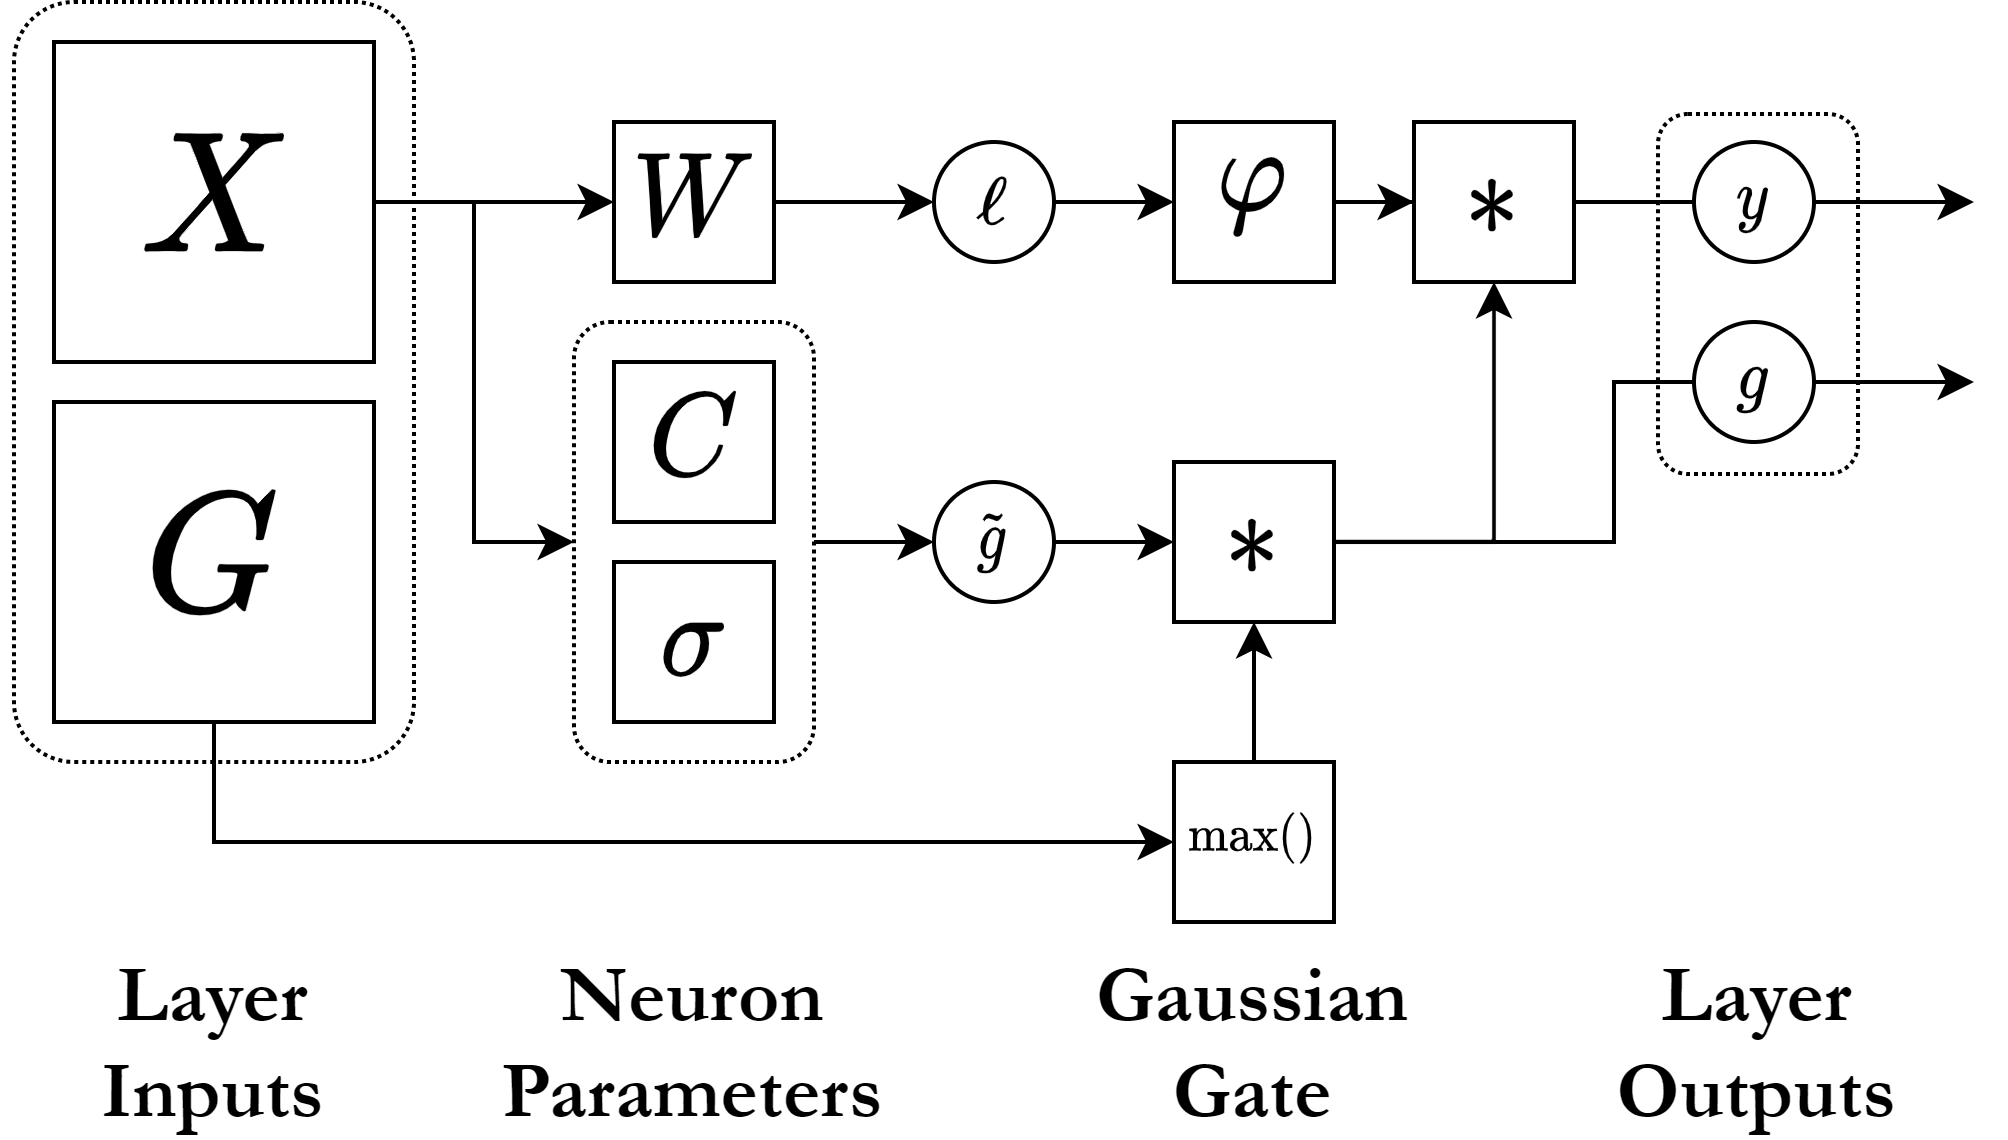
\includegraphics[width=\textwidth]{images/multi-layer-fgn/FGN-Network.png}
    \caption{Illustration of an FGN's output computation when integrated in a neural network. The added Gaussian gate allows for zero activity due to out-of-range inputs to propagate throughout the network. Both $y$ ang $g$ are outputed to the next layer.}
    \label{fig:fgn-layer}
\end{figure}\\
% toy 2D data
\indent To illustrate the difference in behavior between a neural network built form classical neuron compared to a network built from FGNs, consider the two class, two dimensional, non-linearly separable toy dataset in figure \ref{fig:toy-2d-data}. After training two feedforward neural networks, one with FGNs and the other with classical neurons but otherwise identical, figure \ref{fig:toy-2d-activities} shows that, while both networks are able to properly separate the two classes, the FGN network restricts its predictions to zones of the space where the data is present, while the classical network does not. Figure \ref{fig:toy-2d-params} gives additional details on the experiment.

\begin{figure}[!htbp]
    \centering
        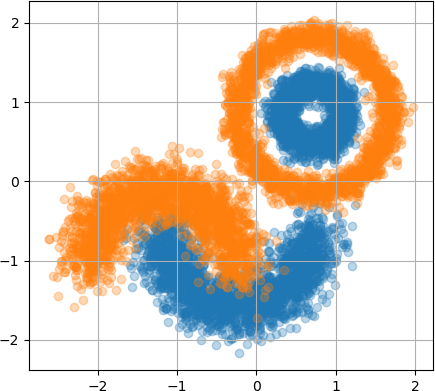
\includegraphics[width=0.66\textwidth]{images/2D-network-toy/2d-toy-data.png}
    \caption{Two class, two dimensional, non-linearly separable toy dataset}
    \label{fig:toy-2d-data}
\end{figure}
\begin{figure}[!htbp]
    \centering
    \begin{subfigure}[t]{0.49\textwidth}
        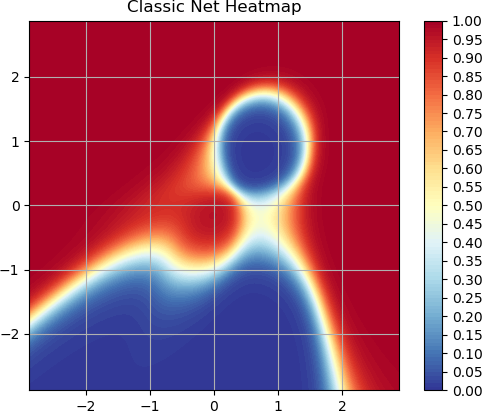
\includegraphics[width=\textwidth]{images/2D-network-toy/classic-heatmap.png}
        % \caption*{}
    \end{subfigure}
    \begin{subfigure}[t]{0.49\textwidth}
        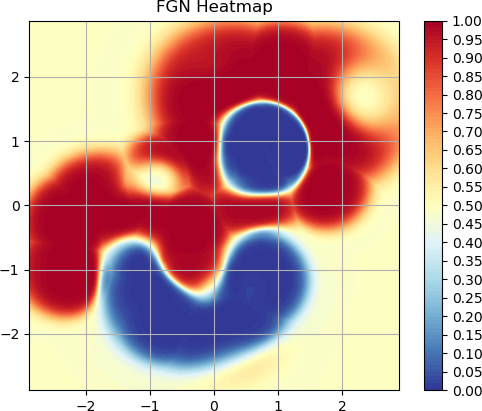
\includegraphics[width=\textwidth]{images/2D-network-toy/fgn-heatmap.png}
        % \caption*{}
    \end{subfigure}
    \caption{Comparison of the activity heatmap between a classical neural network and the same network except using FGNs instead of classical neurons. Both networks separate the data shown in figure \ref{fig:toy-2d-data}, but only the classical network makes predictions far from the data.}
    \label{fig:toy-2d-activities}
\end{figure}
\begin{figure}[!htbp]
    \centering
    \begin{subfigure}[t]{0.49\textwidth}
        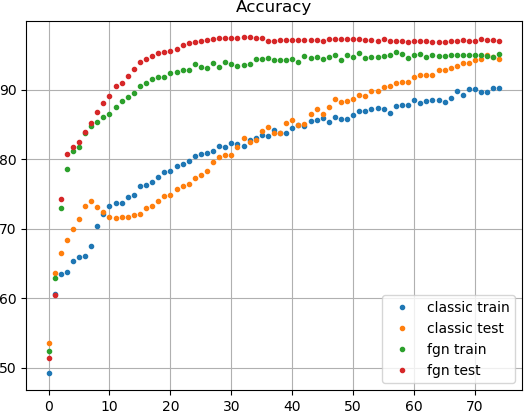
\includegraphics[width=\textwidth]{images/2D-network-toy/training-accuracy.png}
        \caption*{Classic vs FGN training accuracies}
    \end{subfigure}
    \begin{subfigure}[t]{0.49\textwidth}
        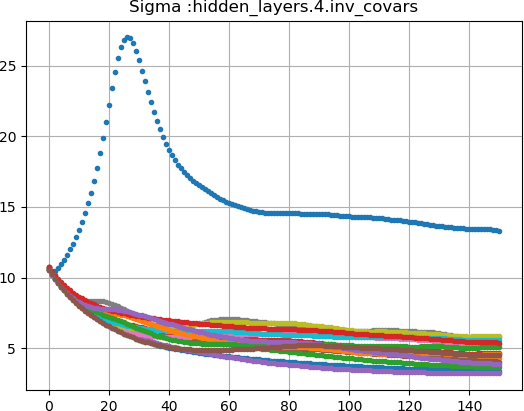
\includegraphics[width=\textwidth]{images/2D-network-toy/sigmas-change.png}
        \caption*{Changes to the network's FGNs ranges}
    \end{subfigure}
    \caption{Network parameters: 32-16 neurons in hidden layers, dropout layers with 1/16 drop rate, spherical range $\sigma$ and 2-norm for the FGN. First FGN layer centers initialized to random data points.}
    \label{fig:toy-2d-params}
\end{figure}
 
\chapter{Experimental Results: FGNs over MNIST}
With the behavior of FGNs verified on toy data, we now test it on real data, with the goal of providing defense against adversarial attacks. The first dataset tested is MNIST, a collection of handwritten digit images by LeCun et al. \cite{lecun-mnisthandwrittendigit-2010}. Three networks will be compared:
\begin{itemize}
    \item A network built with two layers of 64 classical each, with dropout layers with drop rate 0.2 in between each layer.
    \item A network built from FGNs directly converted from the classic network above, with no retraining, and with a range $\sigma=10$ large enough to not modify the behavior over the training data.
    \item The same FGN network as above, but retrained over the data for a single epoch with a tiny $\lambda=10^{-10}$ loss pressure to shrink the ranges $\sigma$.
\end{itemize}
All three networks have over 99\% accuracy over the training data and over 97\% over the validation data. The specific network design choices (size and number of layers) are not relevant to the conclusions drawn, as other designs were tested with similar experimental results. The three networks will be tested over two sets of random images: one built from images with fully randomized pixel values, which have different mean and variance compared MNIST; and the other built from images consisting of shuffled MNIST images, which preserve the mean and variance. Figure \ref{fig:randoms} shows image samples from these two sets.
\begin{figure}[!htbp]
    \centering
    \begin{subfigure}[t]{0.49\textwidth}
        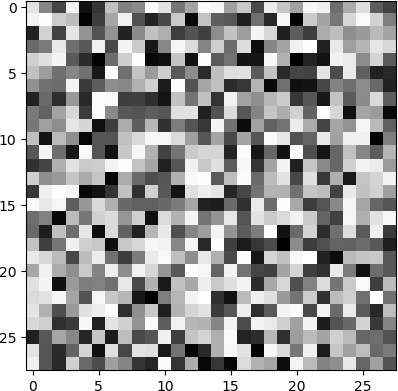
\includegraphics[width=\textwidth]{images/mnist-behavior/MNIST-Sample-random-noise-fixed.png}
        \caption*{Fully random pixels}
    \end{subfigure}
    \begin{subfigure}[t]{0.49\textwidth}
        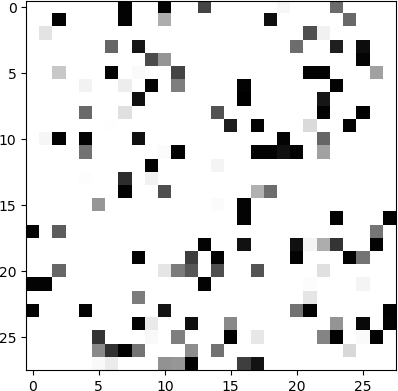
\includegraphics[width=\textwidth]{images/mnist-behavior/MNIST-Sample-random-shuffled-noise-fixed.png}
        \caption*{Shuffled MNIST image}
    \end{subfigure}
    \caption{Samples from the two random images datasets.}
    \label{fig:randoms}
\end{figure}

\section{Behavior of Random Images}
While the classical network has a high accuracy, it also has a high confidence in it's predictions. Over the validation set, over 99\% of its predictions gave one of the ten digit classes a confidence greater that $0.5$ i.e. a majority confidence over all the other classes. In fact most of the predictions are well into the [$0.9,1.0$] confidence range, as shown by figure \ref{fig:classic-mnist}.
\begin{figure}[!htbp]
    \centering
    \begin{subfigure}[t]{0.49\textwidth}
        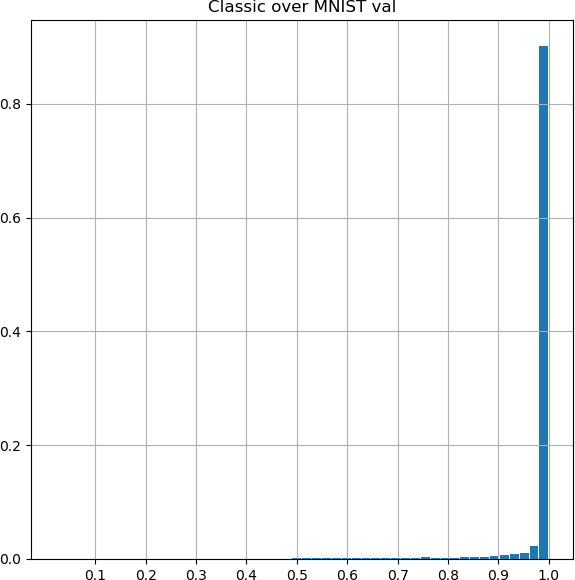
\includegraphics[width=\textwidth]{images/mnist-behavior/classic-hist-val.png}
        % \caption*{}
    \end{subfigure}
    \caption{Histogram of confidences - classic network.}
    \label{fig:classic-mnist}
\end{figure}\\
\indent When the same network is tested over the randomized images sets, the histograms of confidences  \ref{fig:classic-hists} show that a majority of predictions still have above $0.5$ confidence, even though the randomized images are far away in the high dimensional hyper-space from the MNIST images. Figure \ref{fig:classic-preds} shows examples of randomized images, highlighting those given an MNIST digit class with over 0.9 confidence. This is replication of results given in \cite{szegedy2013intriguing}.
\begin{figure}[!htbp]
    \centering
    \begin{subfigure}[t]{0.49\textwidth}
        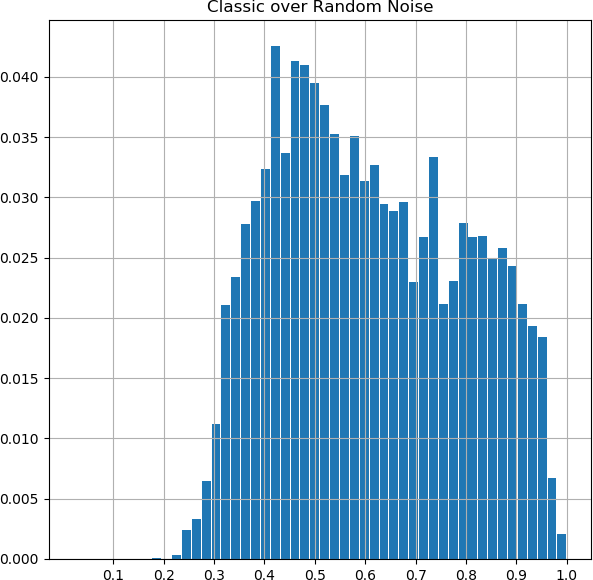
\includegraphics[width=\textwidth]{images/mnist-behavior/classic-hist-random.png}
        \caption*{Over 66\% of confidences $>0.5$}
    \end{subfigure}
    \begin{subfigure}[t]{0.49\textwidth}
        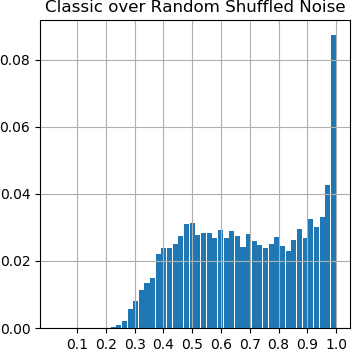
\includegraphics[width=\textwidth]{images/mnist-behavior/classic-hist-shuffled.png}
        \caption*{Over 78\% of confidences $>0.5$}
    \end{subfigure}
    \caption{}
    \label{fig:classic-hists}
\end{figure}
\begin{figure}[!htbp]
    \centering
    \begin{subfigure}[t]{0.49\textwidth}
        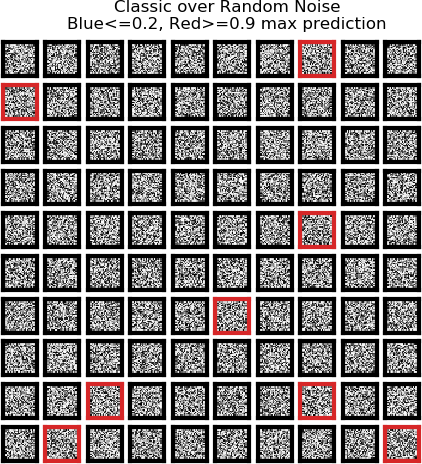
\includegraphics[width=\textwidth]{images/mnist-behavior/classic-pred-random.png}
        % \caption*{}
    \end{subfigure}
    \begin{subfigure}[t]{0.49\textwidth}
        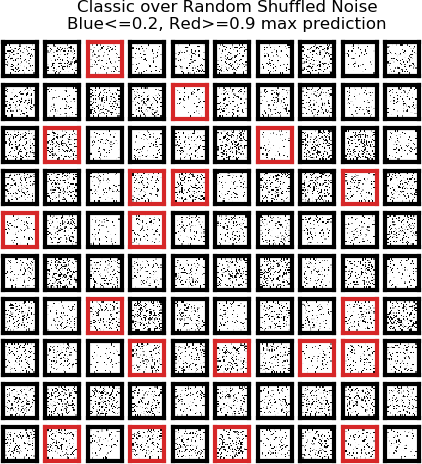
\includegraphics[width=\textwidth]{images/mnist-behavior/classic-pred-shuffled.png}
        % \caption*{}
    \end{subfigure}
    \caption{Sample over-confident predictions made by the classic network.}
    \label{fig:classic-preds}
\end{figure}\\
\indent Be design the converted FGN network does not modify the behavior of the classic network over the MNIST training data. It outputs identical values and the histogram of its prediction confidences over the validation data looks identical to that of classic network shown in figure \ref{fig:classic-mnist}. By contrast, when the converted FGN network is tested over the randomized images sets, the histograms are shifted towards lower values, with fewer confident predictions. These histograms are shown in figure \ref{fig:converted-hist}.
\begin{figure}[!htbp]
    \centering
    \begin{subfigure}[t]{0.49\textwidth}
        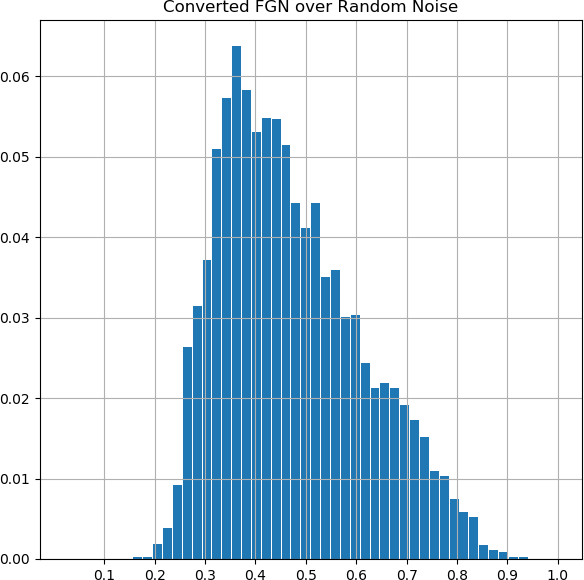
\includegraphics[width=\textwidth]{images/mnist-behavior/converted-hist-random.png}
        \caption*{Over 47\% of confidences $>0.5$}
    \end{subfigure}
    \begin{subfigure}[t]{0.49\textwidth}
        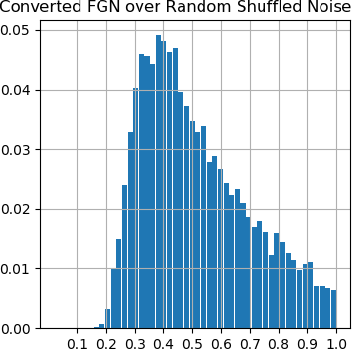
\includegraphics[width=\textwidth]{images/mnist-behavior/converted-hist-shuffled.png}
        \caption*{Over 45\% of confidences $>0.5$}
    \end{subfigure}
    \caption{}
    \label{fig:converted-hist}
\end{figure}\\
\indent Finally, the FGN network is retrained over MNIST for a \emph{single} epoch. The pressure to shrink the ranges $\sigma$ of the network's FNGs, added to the loss function, was a tiny $\lambda=10e^{-10}$. The overall accuracy remains the same (99\% over training data and 97\% over validation data) and still the network outputs extremely confident predictions. The figure \ref{fig:retrained-mnist} is functionally identical to \ref{fig:classic-mnist}. But when this network is tested over the randomized image sets, almost all the predictions are at 0.1, as shown in figure \ref{fig:ret-hist}, meaning the network is actually all zeros, and making no prediction for these randomized images that are far away in the high dimensional hyper-space from the MNIST images. The retrained FGN network is restricting its activity exclusively to zones of the hyper-space in which the training data is present. These zones are still large enough to generalize from the training data to the validation data.
\begin{figure}[!htbp]
    \centering
    \begin{subfigure}[t]{0.49\textwidth}
        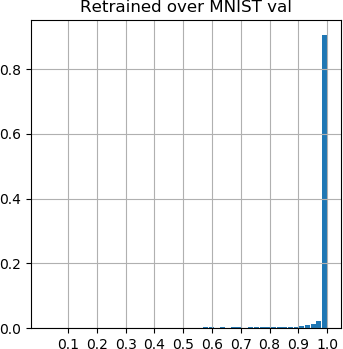
\includegraphics[width=\textwidth]{images/mnist-behavior/retrained-hist-val.png}
        % \caption*{}
    \end{subfigure}
    \caption{Histogram of confidences - retrained FGN network.}
    \label{fig:retrained-mnist}
\end{figure}
\begin{figure}[!htbp]
    \centering
    \begin{subfigure}[t]{0.49\textwidth}
        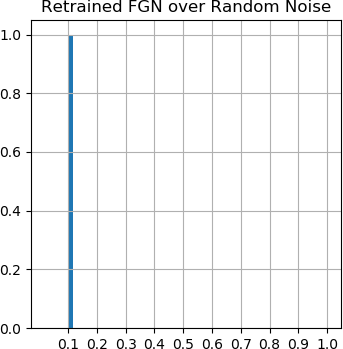
\includegraphics[width=\textwidth]{images/mnist-behavior/retrained-hist-random.png}
        \caption*{0.0\% of of confidences $>0.5$}
    \end{subfigure}
    \begin{subfigure}[t]{0.49\textwidth}
        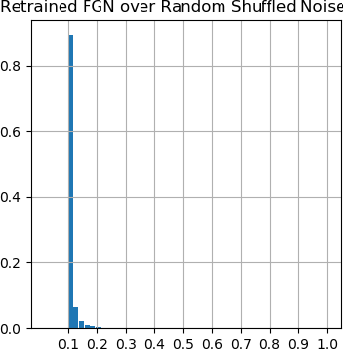
\includegraphics[width=\textwidth]{images/mnist-behavior/retrained-hist-shuffled-fixed.png}
        \caption*{0.05\% of confidences $>0.5$}
    \end{subfigure}
    \caption{}
    \label{fig:ret-hist}
\end{figure}\\
\indent Finally the three networks are tested on the EMNIST dataset, a collection of handwritten letter images by Cohen et al. \cite{cohen2017emnist}, a verification of the FGN behavior to out-of-domain samples. The histograms of the prediction confidences are shown in figure \ref{fig:hist-letters} and tell the same story as above: the classic models makes many confident predictions, the converted FGN network makes fewer, and the retrained FGN network makes none. Samples images are shown in figure \ref{fig:pred-letters}.
\begin{figure}[!htbp]
    \centering
    \begin{subfigure}[t]{0.32\textwidth}
        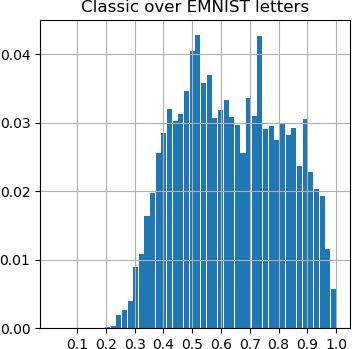
\includegraphics[width=\textwidth]{images/Letters/hist-classic-letters.png}
        \caption*{73\%  of confidences $>0.5$}
    \end{subfigure}
    \begin{subfigure}[t]{0.32\textwidth}
        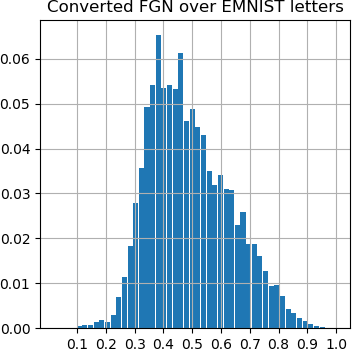
\includegraphics[width=\textwidth]{images/Letters/hist-converted-letters.png}
        \caption*{42\% of confidences $>0.5$}
    \end{subfigure}
    \begin{subfigure}[t]{0.32\textwidth}
        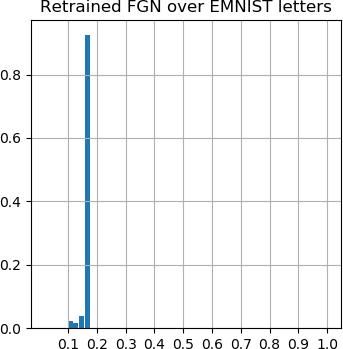
\includegraphics[width=\textwidth]{images/Letters/hist-retrained-letters.png}
        \caption*{0.0\% of confidences $>0.5$}
    \end{subfigure}
    \caption{}
    \label{fig:hist-letters}
\end{figure}
\begin{figure}[!htbp]
    \centering
    \begin{subfigure}[t]{0.32\textwidth}
        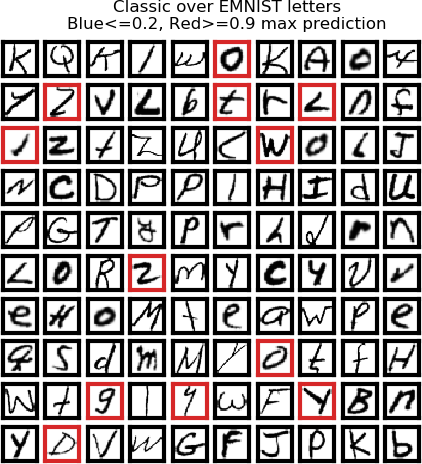
\includegraphics[width=\textwidth]{images/Letters/classic-letters.png}
    \end{subfigure}
    \begin{subfigure}[t]{0.32\textwidth}
        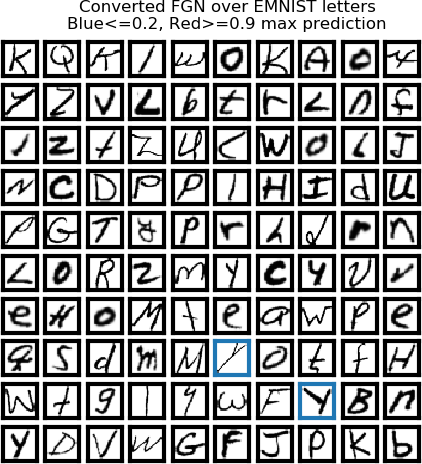
\includegraphics[width=\textwidth]{images/Letters/converted-letters.png}
    \end{subfigure}
    \begin{subfigure}[t]{0.32\textwidth}
        \includegraphics[width=\textwidth]{images/Letters/retrained-letters.png}
    \end{subfigure}
    \caption{Sample EMNIST images with their prediction confidences given by the different networks. Note that some of the confident predictions by the classic network are on images of letters that resemble digits, yet it misses other. Humans would classify all the letter Os as digit zero. By contrast the retrained FGN networks makes no confident predictions for any of the letters, regardless of how close they resemble digits to humans.}
    \label{fig:pred-letters}
\end{figure}

\section{Protection against FGSM attack}
While protection from out-of-domain predictions is a useful feature of FGN networks, it does not guarantee protection from adversarial attacks. 

\chapter{Remaining Work}



%% If you want an introduction in the table of contents, but
%% without its own chapter number, do this:
%% \chapter*{Introduction}
%% \addcontentsline{toc}{chapter}{\numberline{}Introduction}
%% \markboth{Introduction}{INTRODUCTION}

%% Also, to ensure that the bibliography is in the table of
%% contents, do this when you reach the end of the main text:

\backmatter
%% \begin{thebibliography}{n} %(where n is the longest item)
%% \addcontentsline{toc}{chapter}{\numberline{}Bibliography }

\bibliographystyle{IEEEtran}
\bibliography{bibl.bib}


\end{document}